\documentclass{standalone}
\usepackage{tikz}

\begin{document}

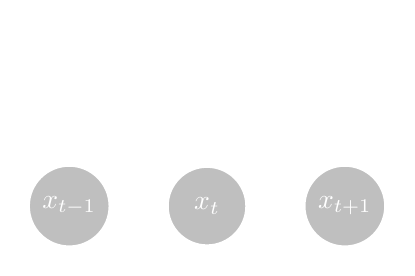
\begin{tikzpicture}[scale=1.5, node distance=1.75cm, every node/.style={circle, draw=white, text=white, minimum size=1cm, thick}]

    % Nodes
    \node[circle, draw=white] (yt1) {$y_{t-1}$};
    \node[circle, draw=white, right of=yt1] (yt) {$y_t$};
    \node[circle, draw=white, right of=yt] (ytp1) {$y_{t+1}$};
    
    \node[circle, draw=white, fill=gray!50, below of=yt1] (xt1) {$x_{t-1}$};
    \node[circle, draw=white, fill=gray!50, below of=yt] (xt) {$x_t$};
    \node[circle, draw=white, fill=gray!50, below of=ytp1] (xtp1) {$x_{t+1}$};
    
    % Edges
    \draw[white, ->] (yt1) -- (yt);
    \draw[white, ->] (yt) -- (ytp1);
    \draw[white, ->] (yt1) -- (xt1);
    \draw[white, ->] (yt) -- (xt);
    \draw[white, ->] (ytp1) -- (xtp1);

\end{tikzpicture}

\end{document}
